\section{Experimental Results}
\label{sec:experiments}

\noindent\textbf{Dataset}.
We perform our training and test on Task~1, the frame-level VAD, of DoTA dataset \cite{9712446}, using only the anomaly class and its temporal boundaries, strictly in the online scenario.
%It contains 4677 videos taken from YouTube, recorded in different countries and with different illumination and weather conditions, with a resolution of $1280 \times 720$.
%We use the original dataset split, which approximately divide the training and validation in $70\%$ and $30\%$.
% , that is the most realistic and most interesting condition from our point of view.

\newcommand{\figsize}{0.8\columnwidth}

\begin{figure}[t!]
\centerline{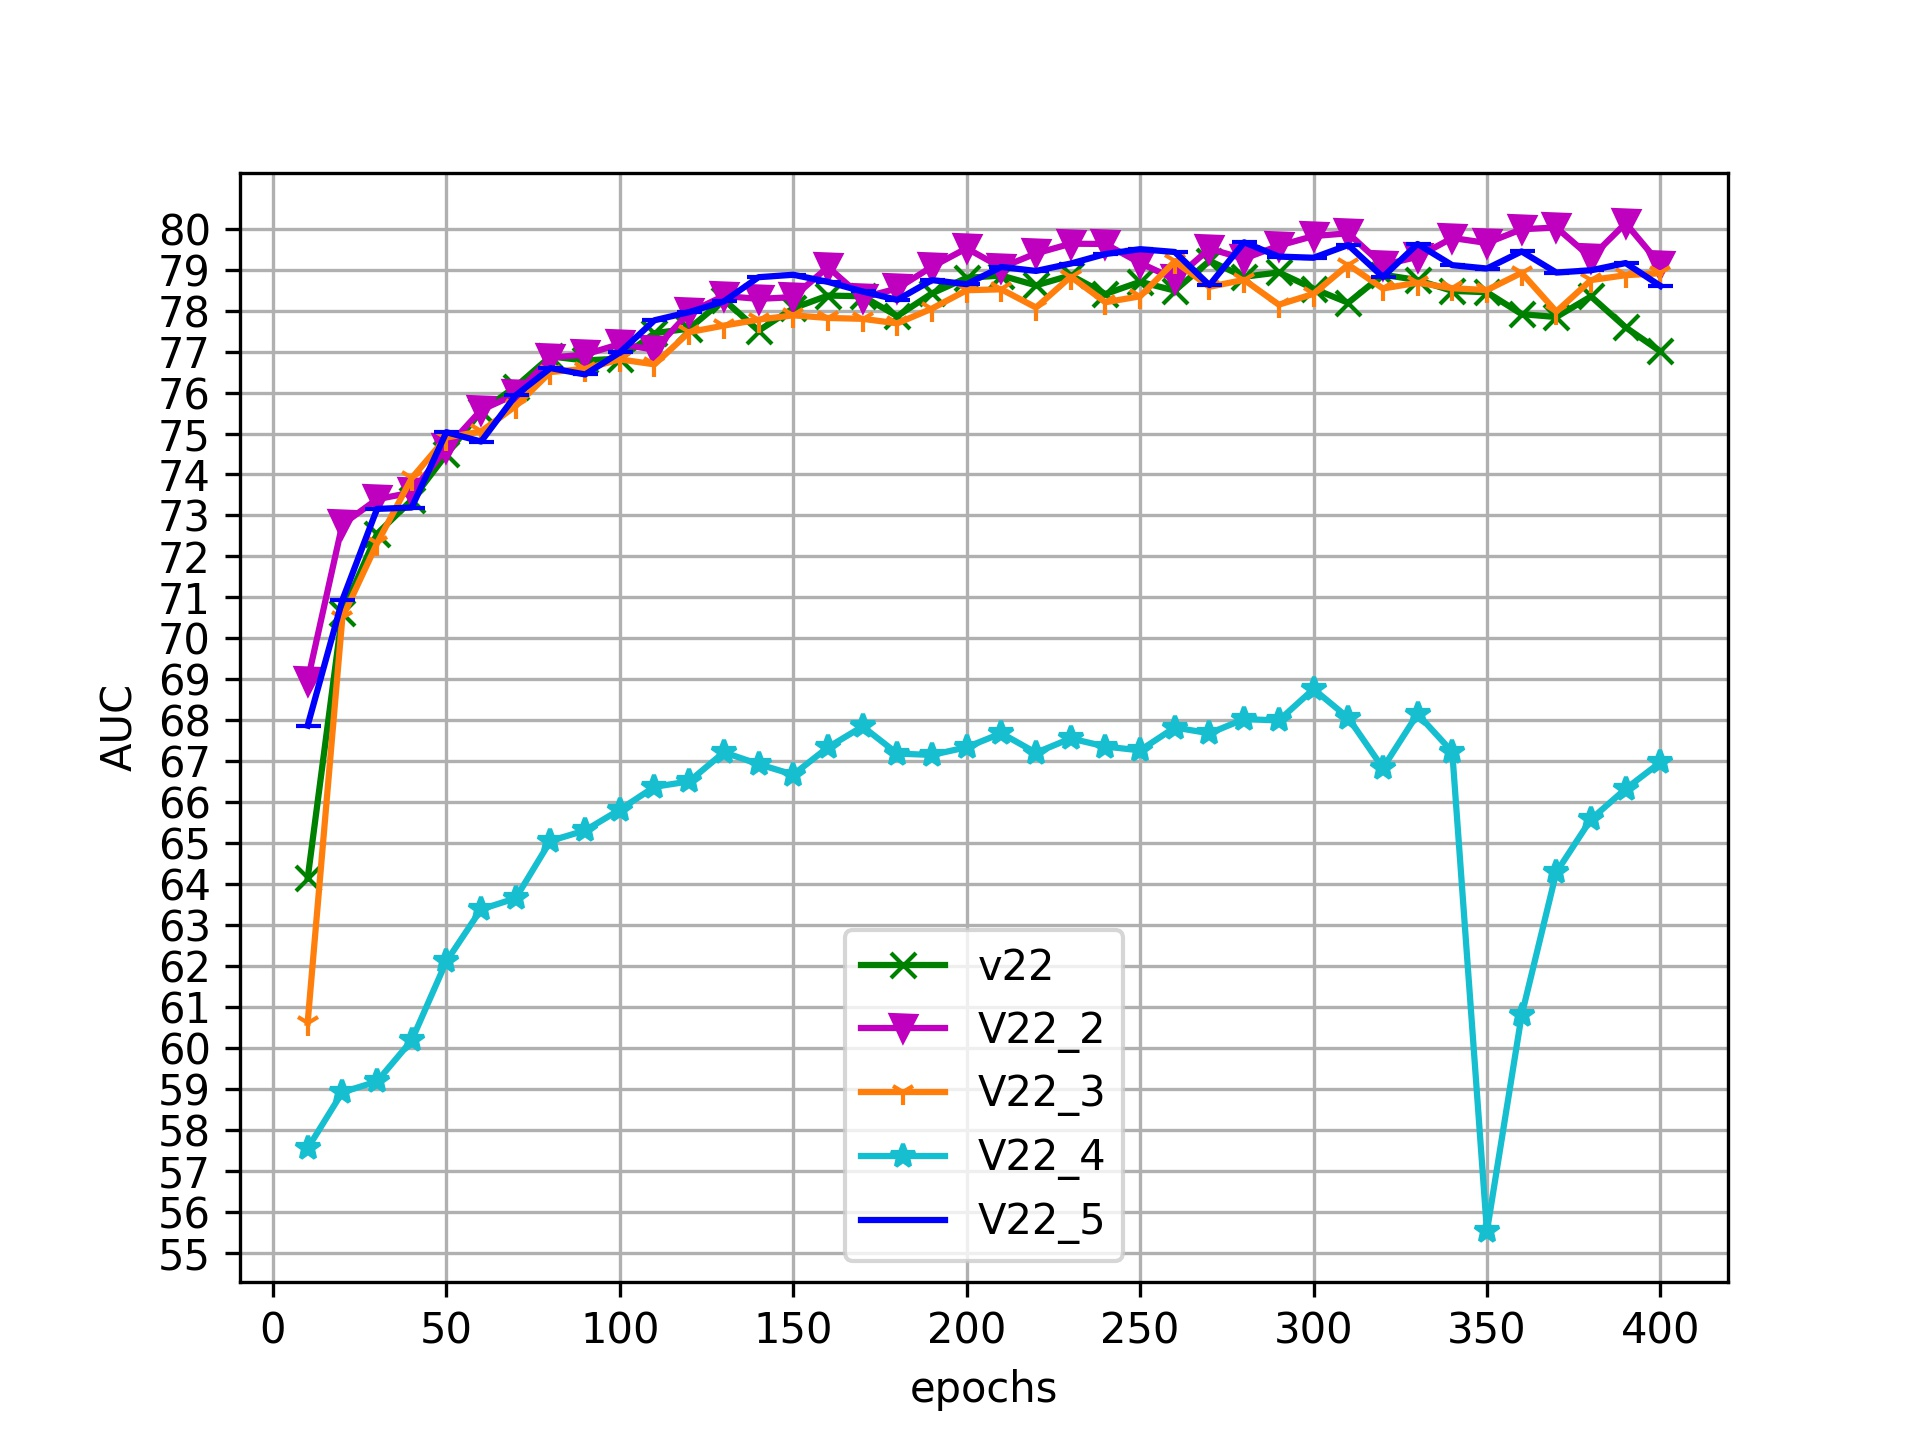
\includegraphics[clip,width=\figsize]{images/exp_1.jpg}}
	\caption{Performance comparison, changing the number of frames ($\mathit{NF}$) in input to the VST (from 1 to 5).}
	\label{fig:num-frames-vst}
\end{figure}


\begin{figure}[t!]
\centerline{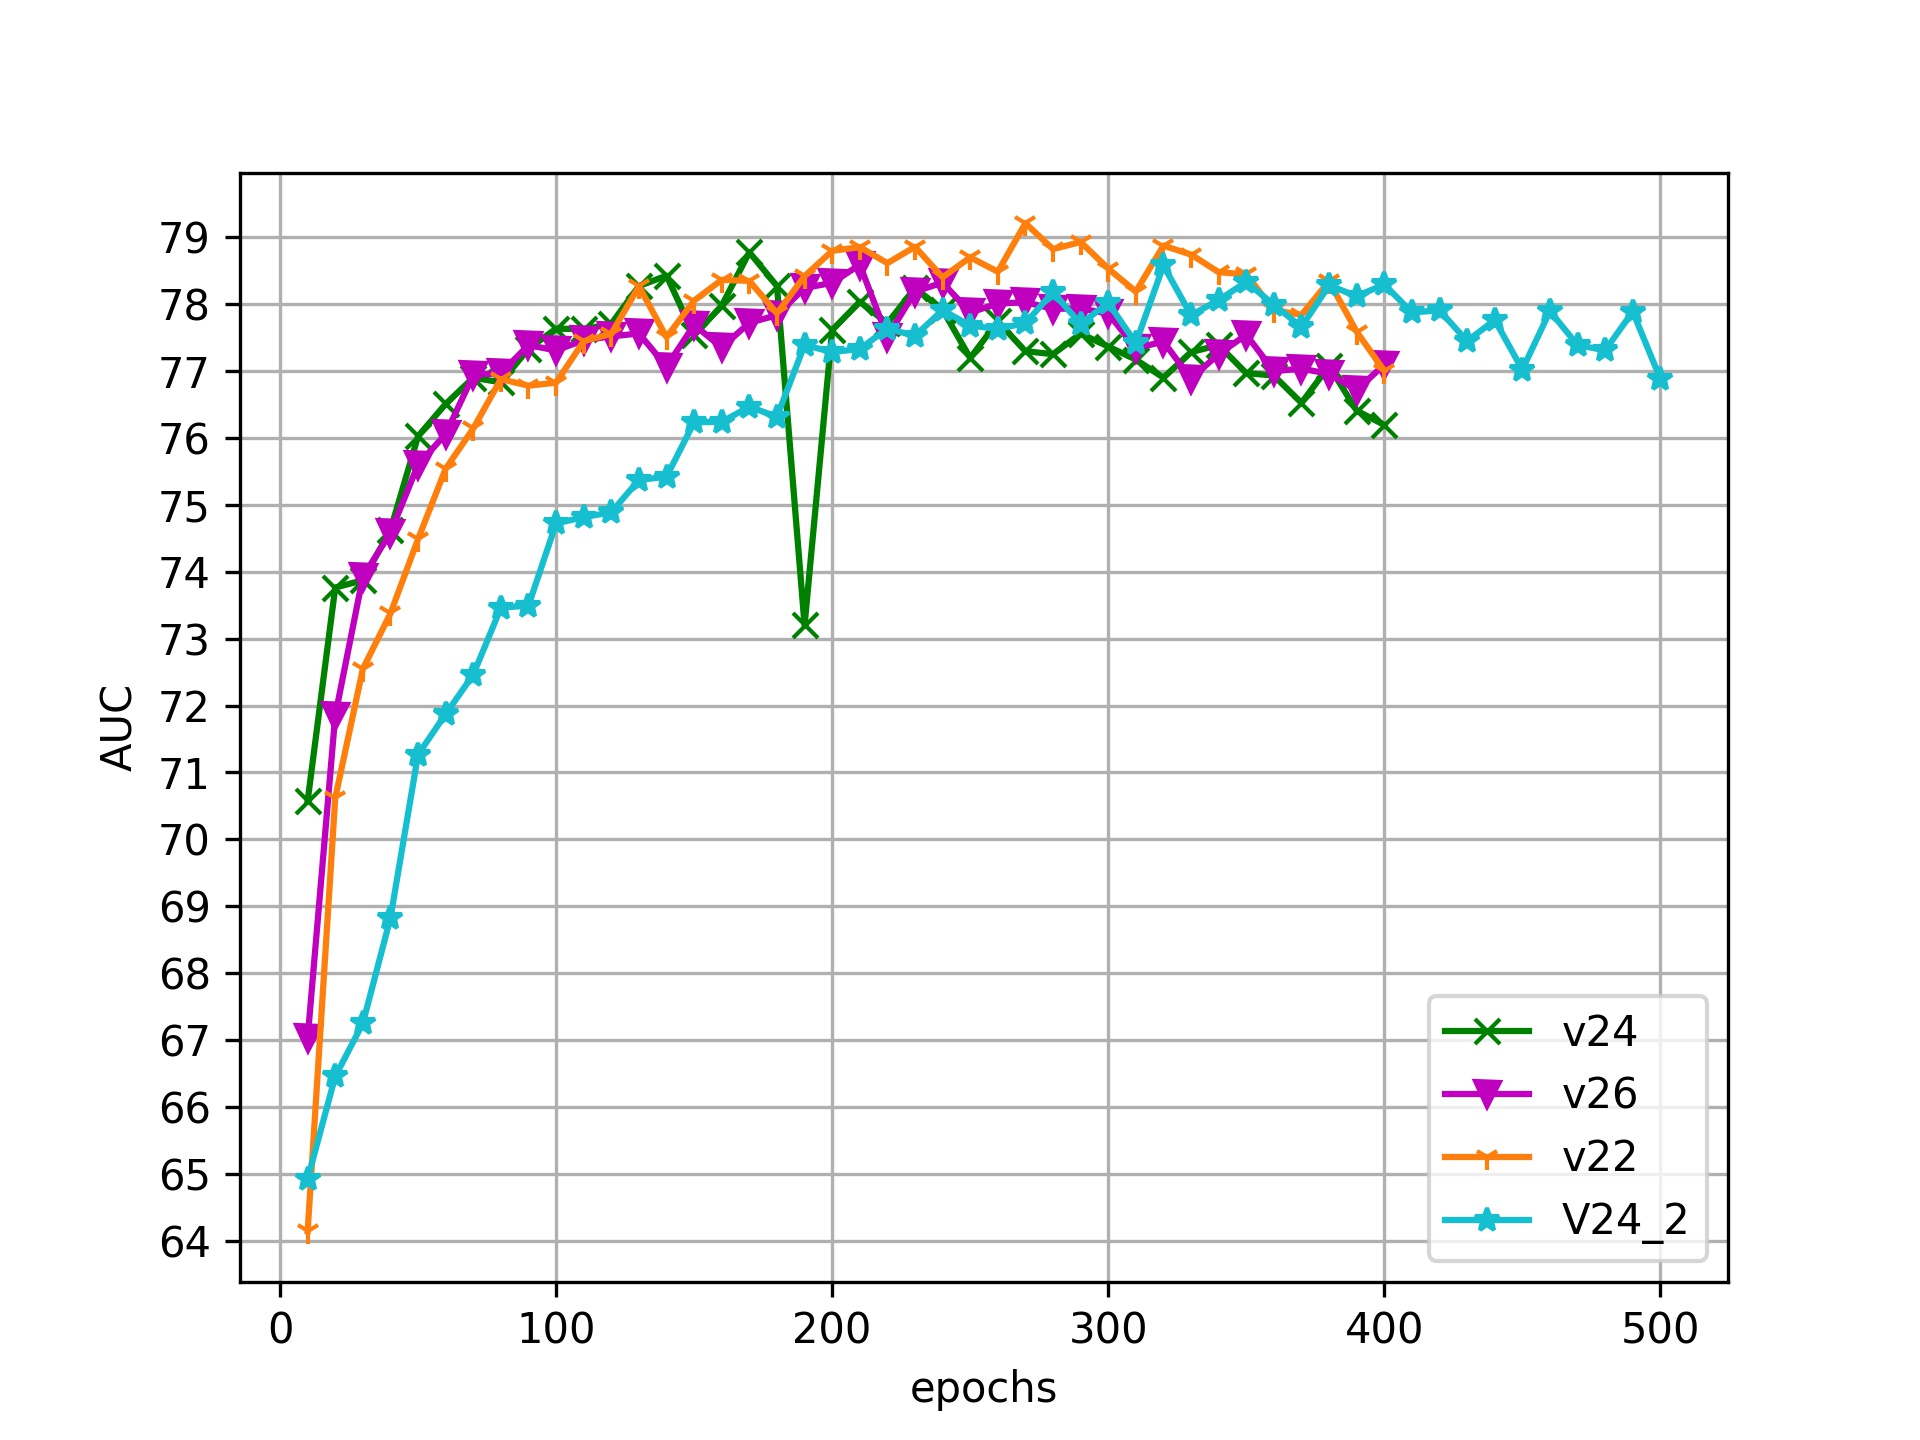
\includegraphics[clip,width=\figsize]{images/exp_2.jpg}}
    % TODO aggiorna caption!
	\caption{Performance comparison, changing the number of LSTM cells (from 0 to 4). ``LSTM (2 cells)'' corresponds to ``$\mathit{NF}=3$''  in Fig.~\ref{fig:num-frames-vst}.}
	\label{fig:num-memory-cells}
\end{figure}

\noindent\textbf{Evaluation Metrics}.
We use the well-known Area Under the Curve (AUC) metric at frame-level, to evaluate how well the model is able to temporally locate the anomaly in the videos.

\noindent\textbf{Training details.}
%The results of the models, with which we compare, are taken from the respective papers.
We perform the training on a single machine with an A100 GPU\@, with Stochastic Gradient Descent (SGD) optimization algorithm, learning rate of 0.0001, momentum of 0.9.
We use SGD instead of Adam because in our experiments the latter led the training to be more unstable, resulting in model diverging after few epochs.
Unless otherwise specified, batch size is 8, input video size is $320 \times 240$, Video Clip Length (VCL), which is the number of frames inside the batch for each video, is 8, LSTM cell number is 2, $\mathit{NF}$ is 3, linear weights are initialized using a uniform distribution, LSTM cells with a (semi-)orthogonal matrix, bias parameters are set to zero and the VST is initialized with a model pretrained on Something-Something v2~\cite{goyal2017something}.
We train using a weighted Cross-Entropy loss to address the issue of imbalanced data within the DoTA dataset, assigning $w_n=0.3$ and $w_a=0.7$ to the normal and anomaly class, respectively following equation reported at the end of Section \ref{sec:theory}.

\begin{figure}[ht!]
\centerline{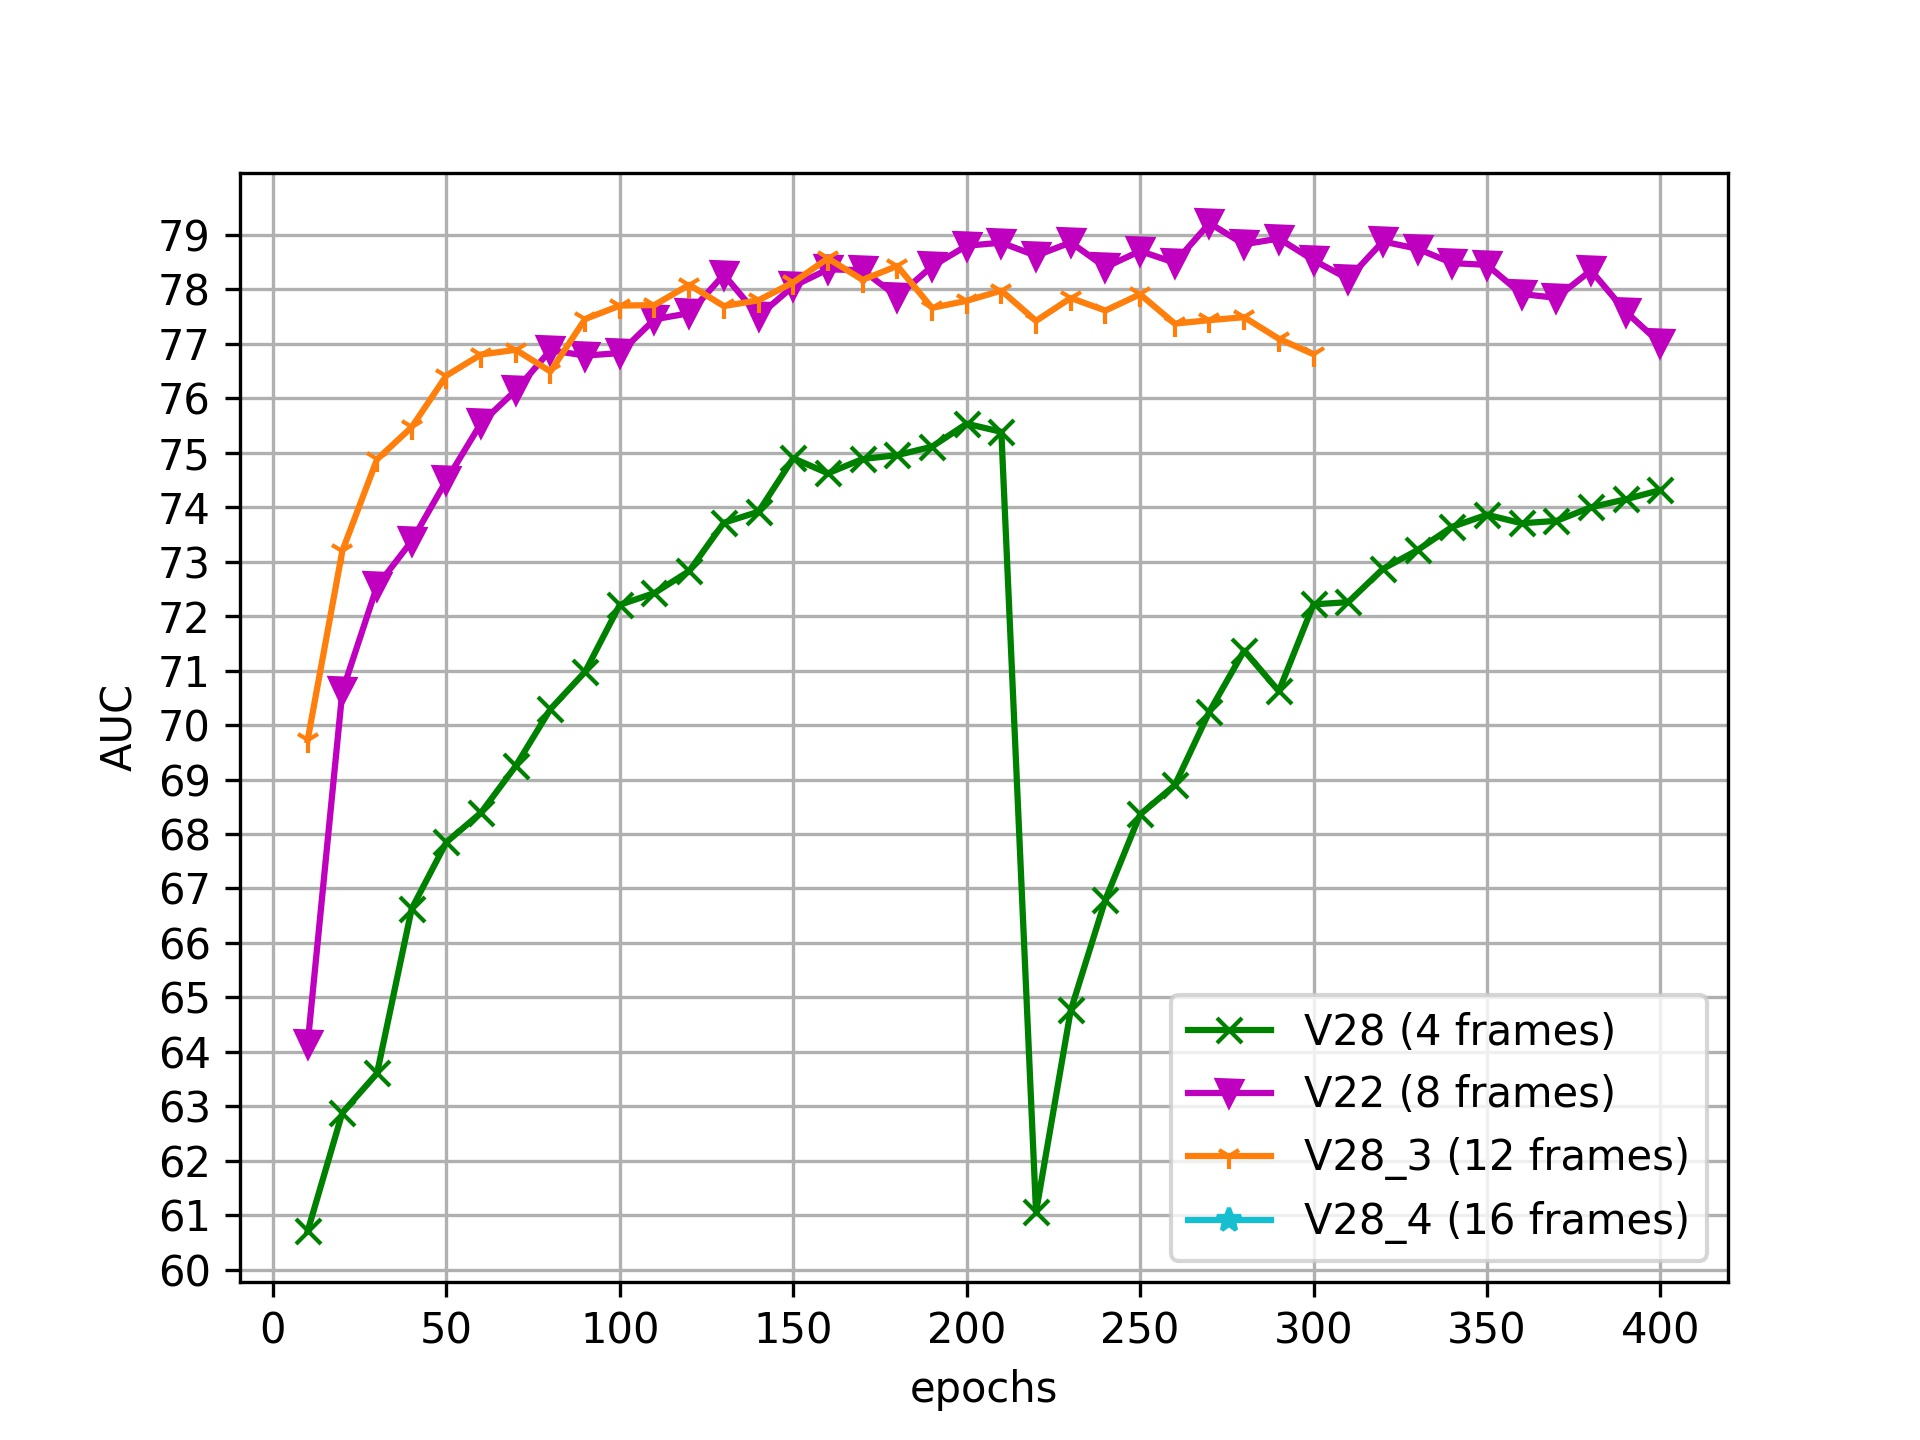
\includegraphics[clip,width=\figsize]{images/exp_3.jpg}}
    \caption{Performance comparison, changing the VCL. The ``8 frames'' configuration corresponds to ``$\mathit{NF}=3$'' in Fig.~\ref{fig:num-frames-vst}.\label{fig:random-batch}}
\end{figure}
\begin{table}[ht!]
	\normalsize
	%\setlength{\tabcolsep}{1.2pt}
	\centering
     \begin{adjustbox}{width=0.5\linewidth}
     \begin{tabular}{!r|^c|^c|^c|}
                \# & Short-term & Long-term & $AUC$ \\
                \hline\hline
                        1 &            &            & 66.53 \\
                        2 & \checkmark &            & 74.46 \\
                        3 &            & \checkmark & 68.76 \\
    \rowstyle{\bfseries}    4 & \checkmark & \checkmark & 79.21 \\
    \end{tabular}
    \end{adjustbox}
    \hspace{0.5em}
	\caption{Performance comparison with and w/out short and long-term memory. Short-term: with ($\mathit{NF}=3$) and w/out ($\mathit{NF}=1$). Long-term: with (2 cells) and w/out (0 cells). }
 % Preliminary results before obtaining best MOVAD configuration.}
	\label{tab:short-vs-long-term-auc}
\end{table}
\begin{table}[ht!]
	\normalsize
	\setlength{\tabcolsep}{4.2pt}
    
	\centerline{
 \begin{adjustbox}{width=0.8\linewidth}
 \begin{tabular}{!r|^l|^l|^c|}
			\# & Method & Input & $AUC$ \\
			\hline\hline
	   	            1 & ConvAE \cite{hasan2016learning} (*)       & Gray                   & 64.3 \\
			        2 & ConvAE \cite{hasan2016learning} (*)       & Flow                   & 66.3 \\
                    3 & ConvLSTMAE \cite{chong2017abnormal} (*)   & Gray                   & 53.8 \\
                    4 & ConvLSTMAE \cite{chong2017abnormal} (*)   & Flow                   & 62.5 \\
                    5 & AnoPred \cite{liu2018future} (*)          & RGB                    & 67.5 \\
                    6 & AnoPred \cite{liu2018future} (*)          & Masked RGB             & 64.8 \\
                    7 & FOL-Ensemble \cite{9712446}  (*)          & RGB + Box + Flow + Ego & 73.0 \\
                    8 & STFE \cite{zhou_spatio-temporal_2022}     & RGB + Flow             & 79.3 \\
            \hline
                    % v22_2
%\rowstyle{\bfseries}9 & Our (MOVAD) & RGB ($320\times240$) &  80.13 \\
                    % v30_3
\rowstyle{\bfseries}9 & Our (MOVAD)                           & RGB ($320\times240$)   & 80.09 \\
                    % v30_2
\rowstyle{\bfseries}10 & Our (MOVAD)                          & RGB ($640\times480$)   & 82.17 \\
\end{tabular}
\end{adjustbox}}
    \hspace{0.5em}
	\caption{Benchmarks of VAD methods on the DoTA dataset. Both MOVAD models are trained with the best configuration of: VCL of 8, 3 LSTM cells and $\mathit{NF}=4$. (Note: Results with (*) are taken from DoTA \cite{liu2018future} paper.}
	\label{tab:sota-vad-auc}
\end{table}
% TODO visualizza anche la colonna OO e VO? (VO and OO columns are not shown because they do not contain anomalous traffic participants)
\begin{table}[ht!]
	\normalsize
	\setlength{\tabcolsep}{3.5pt}
    \begin{adjustbox}{max width=\linewidth}
	\begin{tabular}{
            |!l||^c|^c|^c|^c|^c|^c|^c|^c|^c|}
            \hline
			Model & $ST$ & $AH$ & $LA$ & $OC$ & $TC$ & $VP$ & $VO$ & $OO$ & $UK$ \\
			\hline\hline
                AnoPred \cite{liu2018future}          & 69.9 & 73.6 & 75.2 & 69.7 & 73.5 & 66.3 & N/A & N/A & N/A  \\
                AnoPred \cite{liu2018future} + Mask   & 66.3 & 72.2 & 64.2 & 65.4 & 65.6 & 66.6 & N/A & N/A & N/A \\
                FOL-STD \cite{9712446}                & 67.3 & 77.4 & 71.1 & 68.6 & 69.2 & 65.1 & N/A & N/A & N/A \\
                FOL-Ensemble \cite{9712446}           & 73.3 & 81.2 & 74.0 & 73.4 & 75.1 & 70.1 & N/A & N/A & N/A \\
                % STFE gli manca la colonna VP*!
                % STFE ha dei risultati non molto chiari.
                STFE \cite{zhou_spatio-temporal_2022} & 75.2 & 84.5 & 72.1 & 77.3 & 72.8 & 71.9 & N/A & N/A & N/A \\
                % v22_2 epoca 370
                %\textbf{Our (MOVAD)}                  &  \red{85.6} & \red{84.5} & \red{81.4} & \red{82.8} & \red{84.9} & \textbf{85.8} & \textbf{79.1} & \red{87.4} & \textbf{76.2} & 75.1 & \red{69.9} & 68.4 & 76.6 & \red{75.8} & \red{71.8} & 74.1 & 70.2 & \red{69.4} \\
                % v30_3 560
                \textbf{Our (MOVAD)   }                &  \red{85.6} & \red{85.1} & \red{83.9} & \red{82.2} & \red{85.3} & \textbf{86.2} & \textbf{79.3} & \red{86.7} & \textbf{77.1} \\
                % v30
                %\textbf{Our (MOVAD)} &  \textbf{86.7} & \textbf{86.7} & \textbf{84.1} & \textbf{83.2} & \textbf{86.1} & \textbf{81.9} & 73.2 & \textbf{70.2} & \textbf{74.5} & \textbf{80.0} & \textbf{77.7} & \textbf{75.5} & \textbf{80.1} & \textbf{78.0}  \\
                % v30_2 (epoca 560)
                \textbf{Our (MOVAD) \dag}                &  \textbf{86.6} & \textbf{86.3} & \textbf{84.9} & \textbf{83.7} & \textbf{85.5} & \red{81.6} & \red{77.4} & \textbf{87.9} & \red{73.8} \\
                % v30_2 (epoca 450)
                %\textbf{Our (MOVAD) **}                  &  \textbf{87.2} & \textbf{86.6} & \textbf{85.0} & \textbf{83.8} & \textbf{86.2} & \red{79.1} & \red{77.9} & \red{87.1} & \red{74.1} & 72.8 & \textbf{73.1} & \textbf{75.7} & \textbf{82.2} & \textbf{79.0} & \textbf{74.7} & \textbf{80.3} & \textbf{77.8} & \textbf{72.1} \\
                \hline
            \hline
			Model & $ST*$ & $AH*$ & $LA*$ & $OC*$ & $TC*$ & $VP*$ & $VO*$ & $OO*$ & $UK*$ \\
			\hline\hline
                AnoPred \cite{liu2018future}          & 70.9 & 62.6 & 60.1 & 65.6 & 65.4 & 64.9 & 64.2 & 57.8 & N/A \\
                AnoPred \cite{liu2018future} + Mask   & 72.9 & 63.7 & 60.6 & 66.9 & 65.7 & 64.0 & 58.8 & 59.9 & N/A \\
                FOL-STD \cite{9712446}                & 75.1 & 66.2 & 66.8 & 74.1 & 72.0 & 69.7 & 63.8 & 69.2 & N/A \\
                FOL-Ensemble \cite{9712446}           & \red{77.5} & 69.8 & 68.1 & \red{76.7} & 73.9 & 71.2 & 65.2 & 69.6 & N/A \\
                % STFE gli manca la colonna VP*!
                % STFE ha dei risultati non molto chiari.
                STFE \cite{zhou_spatio-temporal_2022} & \textbf{80.6} & 65.6 & 69.9 & 76.5 & 74.2 & N/A & 75.6 & 70.5 & N/A \\
                % v22_2 epoca 370
                %\textbf{Our (MOVAD)}                  &  \red{85.6} & \red{84.5} & \red{81.4} & \red{82.8} & \red{84.9} & \textbf{85.8} & \textbf{79.1} & \red{87.4} & \textbf{76.2} & 75.1 & \red{69.9} & 68.4 & 76.6 & \red{75.8} & \red{71.8} & 74.1 & 70.2 & \red{69.4} \\
                % v30_3 560
                \textbf{Our (MOVAD)   }                & 72.1 & \red{71.6} & \red{72.3} & 76.5 & \red{75.7} & \red{74.1} & \red{77.9} & \red{71.7} & \red{69.1} \\
                % v30
                %\textbf{Our (MOVAD)} &  \textbf{86.7} & \textbf{86.7} & \textbf{84.1} & \textbf{83.2} & \textbf{86.1} & \textbf{81.9} & 73.2 & \textbf{70.2} & \textbf{74.5} & \textbf{80.0} & \textbf{77.7} & \textbf{75.5} & \textbf{80.1} & \textbf{78.0}  \\
                % v30_2 (epoca 560)
                \textbf{Our (MOVAD) \dag}              & 72.2 & \textbf{74.0} & \textbf{74.8} & \textbf{80.2} & \textbf{79.6} & \textbf{76.8} & \textbf{82.2} & \textbf{78.3} & \textbf{72.9} \\
        \hline
\end{tabular}
    \end{adjustbox}
    \hspace{0.5em}
	\caption{Detection accuracy (AUC) for individual accident categories. ``*'' non-ego anomaly categories. ``\dag'' if input resolution is $640\times480$ instead of $320\times240$. N/A=Not Available. Bold and red values are the best and second-best results.}
	\label{tab:sota-vad-auc-per-class}
\end{table}
% \noindent\textbf{Training details.}
% Since the videos contain a non-equal number of frames, we fixed the number of frames inside the batch for each video (VCL), in order to be able to train the model with a batch size larger than one.
% To make the training as diverse as possible and reduce the effect of overfitting, at each iteration, we randomly choose the starting frame for each video, adjusting the ground-truth accordingly.
% Batch shape is $[B, V, H, W]$, where $B$ is batch size, $V$ is VCL, $H$ and $V$ are height and width, respectively.
% Unless otherwise specified, the following configuration is adopted: input video size is $320 \times 240$, VCL is 8, LSTM cell number is 2, $\mathit{NF}$ is 3, linear weights are initialized using a uniform distribution, the LSTM cells with a (semi-)orthogonal matrix, bias parameters are set to zero and the VST is initialized with a model pretrained on Something-Something v2~\cite{goyal2017something}.
\subsection{Ablation study}
% class weight loss
% 2xsoftmax vs 1x
% learning rate differences (sto finendo l’esperimento con multipli lr)
In this section different configurations will be individually explored and, finally, an optimal setup of MOVAD will be presented in Section \ref{comparison-with-sota}.

\noindent\textbf{Memory modules effectiveness.}
% In this experiment, we study the effects of the memories (short and long). See Table \ref{tab:short-vs-long-term-auc} caption for more details about the configuration.
As shown in Table \ref{tab:short-vs-long-term-auc}, we first tested the effect of both memories.
STMM and LTMM both contribute to enhance the general performance, obtaining the best AUC when both are active, highlighting the need for both. 
%Taking into account the past is always profitable compared to classify the single frame.
%In addition combining these modules allowed to reach the highest AUC, highlighting the need for both.


\noindent\textbf{Short-Term Memory Module.}
\label{Short-Term Memory Module exp}
% v22: numero di frames in input
We decided to design our STMM based on a Video Swin-B architecture, characterized by an embedding dimension of $C = 128$ after the linear projection of the patches. % and layer depths $d_i = \{2, 2, 18, 2\}$, for each $i$-th VST block. %Our experimentation revealed that a larger model (VST-L), was prone to overfitting due to the relatively limited amount of data available for training.
%Our experimentation revealed that lightweight variants (VST-S/T) did not preserve sufficient scene information, as their representations were excessively compressed.
% In this experiment, we study the effects of the past frames in the short-term memory module, varying the number of frames $\mathit{NF}$ processed by the VST at each step.
% The results are displayed in Fig.~\ref{fig:num-frames-vst}.
In Fig.~\ref{fig:num-frames-vst}, results when varying the number of frames $\mathit{NF}$ processed by the VST at each step are displayed.
As expected, taking into account only the current frame is the worst situation, loosing any temporal information and making the training unstable.
This is reasonable: by not having any knowledge of the near past, the STMM leads the LTMM to overfitting since consecutive frames are very similar.
% This is reasonable, as the short-term memory module processes and embeds only the current frame, without any knowledge of the near past, leading the long-term memory module to overfit data since consecutive frames are very similar.
On the contrary, increasing the number of frames generally increase the performance. 
This is true until processing 5 frames, where the effect becomes counterproductive.
As mentioned in section \ref{Long-Term Memory Module descr}, according to our hypotheses, overloading the transformer becomes harmful, as it does not have a mechanism to weight the remote and recent past differently.
Overall, the highest AUC is obtained with 4 frames.
% (no) v23: rand frame order (v17) vs normal
% v29_2, v29, v22: training from scratch vs pretrained (imagenet vs smth2smthv2)

\noindent\textbf{Long-Term Memory Module.}
% posizione dell'lstm senza / prima / dopo / prim + dopo / gru
% v24_4: senza lstm
% v24, v22, v24_2: 1/2/3 # celle lstm
% v26, v26_2, v26_3: 1/2/3 # celle gru
% (no) v27, v27_2: pre + post lstm (1 cell) + saliency (?), pre + post lstm (1 cell)
% In this experiment, we evaluate the long-term memory effect on the classification capability, varying the number of cells from zero (no LSTM at all) to four.
% The results are displayed in Fig.~\ref{fig:num-memory-cells}.
In Fig.~\ref{fig:num-memory-cells} the LTMM on the classification capability are evaluated, varying the number of cells from zero (no LSTM at all) to four.
%We tested also Gated Recurrent Unit (GRU) module instead of LSTM.
%Because the trend is very similar to LSTM, to make the figure easier to read, the GRU results are not shown.
Indeed, having no cells makes training slower in saturating performance and the lowest AUC is reached.
In general, by increasing the number of cells, the maximum AUC is reached slower but it is higher than w/out LSTM.
With 1 cell the performance saturates very quickly, with a slow degradation during the rest of the epochs.
On the other side, 4 cells lead to a very slow saturation w/out reaching the best performance.
The global maximum AUC is reached with 2 cells, even if with just +$0.02$ compared to 3 cells.
Despite this, we prefer the latter configuration, because we think its ability to increase the quality of training in a slower and more continuous way has a better general benefit.
We verified this hypothesis and, in conjunction with $\mathit{NF}=4$ (best configuration in the previous experiment), it permits to obtain higher AUC than with 2 cells.
We speculate this happens because both (3 cells in Fig. \ref{fig:num-memory-cells} and $\mathit{NF}=4$ in Fig. \ref{fig:num-frames-vst}) reach the best AUC at same time (around 400 epochs).

%\noindent\textbf{Saliency module.}
% v25, v22: con/senza/versione ridotta della saliency
%In this experiment, we evaluate the effect of the saliency branch.

\noindent\textbf{Video clip length (VCL).}
% v22, v28: random_batch 4/8/12/16/20/24: describi la modalità di addestramento -> per usare un batch size > 1 si è scelto di selezionare un numero max di frame da elaborare a ogni iterazione. per aggiungere diversità al training, il punto di inizio per ogni video viene scelto in modo casuale a ogni iterazione, adattando di conseguenza il ground-truth
% In this experiment, we evaluate the effect of the VCL (see training details paragraph), varying from 4 to 16.
% In Fig.~\ref{fig:random-batch}, the results are shown.
In Fig.~\ref{fig:random-batch}, different values of VCL are explored.
The worst and most unstable training is obtained with 4 frames, probably because they are too few to exploit the long-term memory effect of LSTM cells.
Increasing VCL permits to saturate performance quicker, but a value too high (like 12 or 16) tends to produce a lower AUC overall.
In fact, the highest AUC is obtained using 8 frames as VCL, which represents a good trade-off between enlarging clip size and exploiting LSTM cells, while avoiding overfitting due to consecutive frames being too similar to each other.

\subsection{Comparison with the state of the art}
\label{comparison-with-sota}
% input shape
% versione finale vs resto del mondo su dota, and: 
%   - Phantom: https://paperswithcode.com/paper/approaches-toward-physical-and-general-video
%   - ShanghaiTech: https://paperswithcode.com/sota/anomaly-detection-on-shanghaitech
%   - CUHK Avenue: https://paperswithcode.com/sota/anomaly-detection-on-chuk-avenue
%   - UCSD Ped2: https://paperswithcode.com/sota/abnormal-event-detection-in-video-on-ucsd
Finally, in Table \ref{tab:sota-vad-auc} we compare MOVAD (with $320\times240$ and $640\times480$ input videos size) with state-of-the-art (SOTA) models.
The training of MOVAD followed the best configuration found using information obtained through ablation studies: VCL of 8, 3 LSTM cells and $\mathit{NF}=4$.
% we have chosen the best configuration for MOVAD.
% Both our models are trained with the best configuration of: VCL of 8, 3 LSTM cells and $\mathit{NF}=4$.
Both MOVAD configurations surpass the SOTA models.
Our best MOVAD surpasses SOTA by +$2.87$ AUC, reaching the highest value of $82.17\%$ AUC.
Table \ref{tab:sota-vad-auc-per-class} shows results per class, grouped by ego and non-ego anomaly categories (see \cite{9712446} for explanation of classes).
It is worth to note that, unlike previous SOTA models, our model also processes without any problem videos in which traffic participants are not present or visible \vnote{, given that it does not need to process bounding boxes}.
For this reason, the table shows results also for ego-involved classes VO (vehicle-obstacle collision) and OO (oncoming out-of-control).
%VB: Potrebbe servire come confronto per il numero parametri e flops
%sembra non riesca a calcolare i flops della rnn però
%| module                    | #parameters or shape   | #flops     |
%|:--------------------------|:-----------------------|:-----------|
%| model                     | 0.144G                 | 0.208T     |
%|  rnn                      |  16.794M               |  0         |
%|   rnn.weight_ih_l0        |   (4096, 1024)         |            |
%|   rnn.weight_hh_l0        |   (4096, 1024)         |            |
%|   rnn.bias_ih_l0          |   (4096,)              |            |
%|   rnn.bias_hh_l0          |   (4096,)              |            |
%|   rnn.weight_ih_l1        |   (4096, 1024)         |            |
%|   rnn.weight_hh_l1        |   (4096, 1024)         |            |
%|   rnn.bias_ih_l1          |   (4096,)              |            |
%|   rnn.bias_hh_l1          |   (4096,)              |            |
%|  rnn_bn                   |  2.048K                |  5.12K     |
%|   rnn_bn.weight           |   (1024,)              |            |
%|   rnn_bn.bias             |   (1024,)              |            |
%|  lin1                     |  37.75M                |  37.749M   |
%|   lin1.weight             |   (1024, 36864)        |            |
%|   lin1.bias               |   (1024,)              |            |
%|  lin2                     |  1.05M                 |  1.049M    |
%|   lin2.weight             |   (1024, 1024)         |            |
%|   lin2.bias               |   (1024,)              |            |
%|  lin3                     |  2.05K                 |  2.048K    |
%|   lin3.weight             |   (2, 1024)            |            |
%|   lin3.bias               |   (2,)                 |            |
%|  bn                       |  73.728K               |  0.184M    |
%|   bn.weight               |   (36864,)             |            |
%|   bn.bias                 |   (36864,)             |            |
%|  model                    |  88.656M               |  0.208T    |
%|   model.patch_embed       |   12.672K              |   0.496G   |
%|    model.patch_embed.proj |    12.416K             |    0.472G  |
%|    model.patch_embed.norm |    0.256K              |    24.576M |
%|   model.layers            |   88.641M              |   0.208T   |
%|    model.layers.0         |    0.571M              |    18.801G |
%|    model.layers.1         |    2.19M               |    17.997G |
%|    model.layers.2         |    60.353M             |    0.153T  |
%|    model.layers.3.blocks  |    25.528M             |    17.831G |
%|   model.norm              |   2.048K               |   3.072M   |
%|    model.norm.weight      |    (1024,)             |            |
%|    model.norm.bias        |    (1024,)             |            |